\chapter{Backgroud}

 As the ORBM builds on the previous work of Restricted Boltzmann Machines and Sigmoid Belief networks, the concepts and previous work in source separation, generative models as well as background on RBMs and Sigmoid Belief Networks need to be introduced.


\section{Generative Models and Source Separation}

Generative models are a powerful way to model data.
\todowording{
(TODO-GRAB-THOSE-GENERATIVE-MODEL-USES-CITATIONS) Basically justify generative models.}

The ORBM proposed in this project aims to represent data generated by two indepedanlty acting causes and does so by combining two existing generative models, the Restricted Boltzmann Machine, and the Sigmoid Belief Network.

\subsection{Terminology in Generative Models observable and hidden variables}

Generative models are comprised of variables, often referred to as units. Some of these variables are observed, that is their state is known. These are often referred to as the `visible` units and are used to represent the training data. For example in the image domain, the visible units correspond to the pixels of the image.

The variables that are not observed, are latent variables, often referred to as `hidden units` as they are not observed.

Connections between units are used to encode relationships between the variables, where the relationship may be causal, such as in a Sigmoid Belief network or an encoding/representation in the Restricted Boltzmann Machine.

Collections of units, are often referred to as `patterns` or `vectors` in that they are represented by a vector or pattern of bits. For instance in the context of an image, the visible pattern would be the pixels of the image ravelled into a one dimensional vector.


\subsection{PGMs as a tool reasoning about generative models}
\todo%
Probalistic Graphical Models or PGMs for short, are an expressive way to represent a collection of related, stochastic variables. If the graph is directed then the edges represent causation, this is also referred to a Bayesian network. Conversely, if the graph was undirected then edges represent a dependancy or mapping. Throughout this report, RBMs, Sigmoid Belief Networks and the proposed ORBM will be shown in this format.

Figure \ref{F:PGM-example} shows an abstract example of a directed PGM, where B is the underlying cause of A, we cannot observe B directly, instead it's state is represented as a `belief` or a probability of being in a given state.

\begin{figure}[h]
\begin{center}
  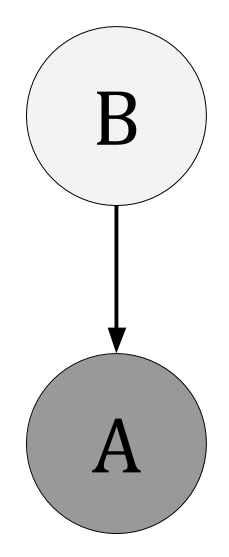
\includegraphics[width = 0.1\textwidth]{Assets/PGM_Example_1.png}
\caption{An example PGM, showing an observed variable `A` and it's hidden cause `B`.}
\label{F:PGM-example}
\end{center}
\end{figure}

\section{Sampling and inverting the model}
Sampling is the process of drawing samples from a distribution. It is used when the distrubtion we want samples from is intractable to calculate analytically. Sampling is required to train generative models, as often the gradient to be climbed/descended involves calculating a probability in the
generative model.
\todo%
\begin{itemize}
  \item Inference is the process of given reasoning about what we do not know given that of which we do know.
  \item In a Generative Model this amounts to the Posterior
\end{itemize}

\subsection{Gibbs sampling, a subset of Markov Chain Monte Carlo}

\begin{itemize}
  \item The importance of Markov Chains and mixing time are crutial in this project
\end{itemize}

Gibbs sampling is a special case of Markov Chain Monte Carlo, a technique for drawing sampling from a complex distribution. The probability mass (the joint distribution) of a generative model is a common use case for Gibbs sampling.

Gibbs sampling explores the desired probability distribution, taking samples of that distributions state, allowing iterations of exploration between drawing of a sample to ensure that the samples are independant. The process of taking a step between states is referred to as a Gibbs iteration.

Gibbs sampling is used for performing inference in the RBMs, Sigmoid Belief Networks and in the ORBM. The mixing time, that is how many Gibbs iterations are needed to reach a satisfactory sample is an important part issue in the ORBM, in that more than one may be required.

\subsubsection{Mixing Time}
MCMC methods require a `mixing` phase to ensure convergence, that is that the sample is being drawn from a representative part of the desired distribution. This is part of the trade off the ORBM attempts to make, as a mixing time is introduced that is not present in the RBM.

  \subsection{Reconstructions, visualising what the model has learnt}

  Generative Models can create an internal representation given an input. They can also generate a faux input given an internal representation. Performing one Gibbs iteration, that is sampling from the hidden units given an input $ P(\tilde{h}|\tilde{v}) $ and then taking the generated hidden state and generating a faux input. The model tries to reconstruct the input.

  \subsubsection{Ancestral Sampling or fanstasies of the model}
  \todo%
  In the same way that a generative model uses reconstructions to try and recreate the  supplied input based purely on how it's represented that input, performing many, many (greater than 100) Gibbs iterations with no input pattern clamped allows the reconstructions to explore the probability mass that the model has built up during training. Sampling from these wanderings creates what are refferred to as `fantasies` or `dreams`. These give a sense of what the model has learnt, and can act a smoke test for if the model has actually capture anything.
  (TODO-CITE-PAPER-WITH-MNIST-DREAM-EVALUATION, they were crappy).

  \section{An intractable model for causes}
    \subsection{Sigmoid Belief Networks}
    \todo%

    The ORBM relies on the Sigmoid Belief Network to capture the causation. The Sigmoid Belief Network is composed of units with weights and a sigmoid activation function, akin to that of a perceptron linear threshold unit/Perceptron. The probability of a node being `on` is found by taking the weighted sum of all input to that node and applying a Sigmoid function or another activation function that ensures a values between $0$ and $1$.

    Belief Networks appear to be an intuitive way to model data in machine learning, as rich dependancies often present in real data can be expressed in it's architecture. Nodes in the network represent binary variables which are dependent on ancestor nodes, the degree of which is encoded in a weight on a directed edge between them.

    Performing inference in a Sigmoid Belief network would allow source separation in that each hidden unit could represent a cause. Meaning if a causes state could be inferred from an input item, individual causes could be examined for an input. For example if the input was an n by n image, the Sigmoid Belief Net makes the assumption that each pixel has an independent cause.

    Despite the Sigmoid Belief Network being expressive and providing a succinct encoding of inter-variable dependancies, the expressiveness is too rich such that performing inference is intractable. There do exist algorithms for performing inference in Sigmoid Belief Networks. For instance, the Belief Propagation algorithm \todocite{The paper where BP/Sum Prod proposed} operates on this encoding, calculating the probabilities of a given network state (i.e. the state of all the variables).  Belief Propagation is intractable to use as the number of variables grow \todocite{ the paper explaining intractable for belief prop}.

    This intractability arises from the Sigmoid Nets richness and the `explaining away effect`. Inference is required for training generative models making Sigmoid Belief Networks impractical to train. \todocite{It has been done, link to paper where they do it.}

    \subsection{Explaining Away creates a trade off between richness and tractability}
    \todo%
    The power of the Belief Network is also it's weakness, a rich structure that models a system of interest inherently has dependancies. In its minimal case explaining away can be seen in a 3 node network popularised by \todocite{AI-A-MODERN-APPROACH-TODO. TODO-GRAPHIC} as shown in figure \ref{F:Explaining-Away}. Each of the nodes represents a binary state. For instance $Burglar = 1$ means that the person owning the \texttt{Alarm} has been burgled. Also note how the connections between the units have arrows, this is causal.

    \begin{figure}[h]
    \begin{center}
      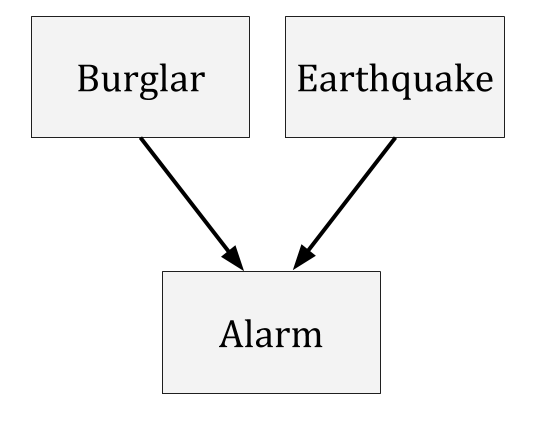
\includegraphics[width = 0.6\textwidth]{Assets/Explaining_Away.png}
    \caption{The famous Burglar, Earthquake, Alarm network showing a minimal case of explaining away.}
    \label{F:Explaining-Away}
    \end{center}
    \end{figure}


    In the network shown in figure \ref{F:Explaining-Away}, knowledge of the \texttt{Alarm} creates a dependance between \texttt{Burglar} and \texttt{Earthqaukes}. For instance, say the Alarm has gone off and we know an earthquake has occurred, our belief in being burgled decreases. The dependance in belief networks means that sampling from the network requires a longer Markov Chain to mix, as changing the value of \texttt{Earthquake}, effects the value of \texttt{Burglar}. \todowording{In a network with many connected nodes the dependence introduced makes sampling take longer. In the context of images, where there may be upwards of 1000 observable values, all with different dependancies this is intractable.}

  \subsection{Boltzmann Machines}

A Boltzmann machine \todocite{Cite the Harmonium, markov field and Hopfield for deterministic example...}  has qualities in common with Belief Networks. Both are generative models with their nodes having probabilities of being active based on neighboring nodes. Connections between nodes have associated weights as shown in figure \ref{F:Boltzmann-Machine}. These weights are symmetric.
\todowording{Unlike a Belief Network, a Boltzmann Machine is a undirected network that allows cycles and thus more complex data can be captured.}

  \todowording{Connections between nodes no longer encode causal information, instead a depedancy, the difference being that a connection encodes a relationship as they are not directed.}

  \begin{figure}[h]
  \begin{center}
    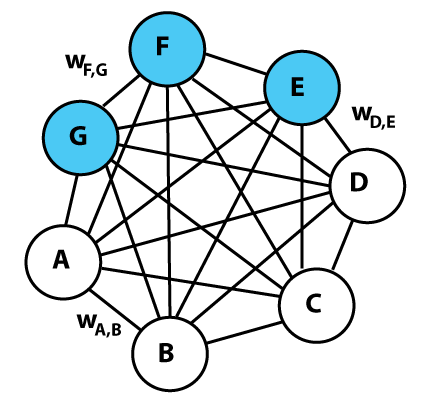
\includegraphics[width = 0.6\textwidth]{Assets/Boltzmann_Machine.png}
  \caption{A Boltzmann Machine, the blue shaded nodes representing the observed variables, and the non-shaded nodes the latent variables.}
  \label{F:Boltzmann-Machine}
  \end{center}
  \end{figure}

  Performing gibbs sampling appears trivial in a Boltzmann Machine, in that to find the probability of a given unit being active a weighted input to that node is passed through a sigmoid function. However, in practice the recurrent nature of Boltzmann Machines makes sampling intractable.

  \todocite{TODO-REFENCE-PAPER-OF-THIS The Boltzmann Machine was shown, given an unreasonable amount of time, to be able to perform better than the state of the art at the time.}


  \section{The Current Approach: A Strong assumption}

  \subsection{Restricted Boltzmann Machines}

  While Boltzmann Machines are impractical to train and sample from as networks grow in size \todocite{Need to cite this\ldots} their architecture can be altered to alieviate these shortcomings. The restriction, proposed by \todocite{Hinton, a proper cite} requires the network to be bipartite, where connections are forbidden between the layer of hidden units and the layer of visible units repectively.

  An example Restricted Boltzmann Machine architecture is shown in figure \ref{F:Restricted-Boltzmann-Machine}. The affect of the restriction is that inference can be tractably computed, as the latent variables no longer become dependant given the observed variables.

  For example in figure \ref{F:Restricted-Boltzmann-Machine} the hidden unit $h_1$ is not dependant on $h_2$ wether or not we know anything about the visible units. This is the opposite of a Sigmoid Belief Network where knowledge of the visible units makes the hidden units dependant. The RBMs nature removes the recurence present in Boltzmann Machines. This reduces the expresiveness of the network but makes the RBM useable in practice. \todocite{The paper about Boltzmann Machines being really good when actually left to find solution.}

  \begin{figure}[h]
  \begin{center}
    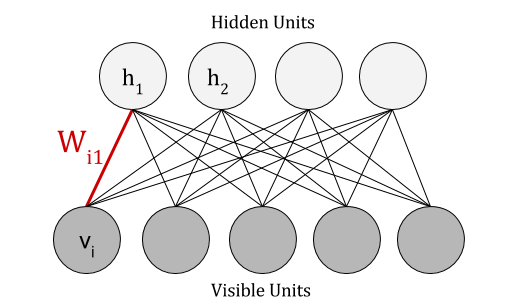
\includegraphics[width = 0.6\textwidth]{Assets/RBM_Example.png}
  \caption{An example Restricted Boltzmann Machine with four hidden units, and five visible units. Note that the edges between units are not directed - representing a dependency not a cause. }
  \label{F:Restricted-Boltzmann-Machine}
  \end{center}
  \end{figure}


  \todo%
  Talk about how Gibbs sampling in RBMs allows us to approximately sample from the hidden (unknown/representation) given the visible (known/input data).
  \todo%

  Hinton TODO-REFERENCE-THE-PAPER proposed a restriction by way of assumption to the Boltzmann Machine that makes it tractable to sample from and therefore train. Boltzmann Machines of this architecture are referred to as Restricted Boltzmann Machines, or RBMs for short.

  The assumption being that the observable and latent variables are independant respectively, enforcing a two layer, fully connected bipartide structure.

    \subsubsection{Tractable Training - Contrastive Divergence}
    Hinton TODO-CITE-CLASSIC-PAPER proposed Contrastive Divergence as a method for training RBMs efficiently. The algorithm leverages the now tractable wake phase because $P(h|v)$ is efficeint to compute. However the free or sleep phase required another restriction where the network is only left to its own dynamics can be limited to only one iteration and still perform well. TODO-CITE-CD-PAPER

  The observed variables are often referred to as the visible units, and will be so forth in this report. The latent variables are often referred to as the hidden units, and will be so forth in this report. Therefore the Restricted Boltzmann machine transforms some visible unit into a hidden representation. These two layers of units can be thought of as vectors of binary values, referred to as $ v $ and $ h $ for visible and hidden layers respectively.

  This restriction allows an efficient calculation of the Wake Phase of generative model learning, as the $ P(h|v) $ can be calculated as a simple weighted sum passed through a sigmoid followed by a bernouli trial where the probability of being $1$ is equal to the result of sigmoid.



  \subsection{Deep Learning}

    \begin{itemize}
      \item Discuss deep learning as there are clear parallels to Deep Belief Networks and the new approach
      \item in paritcular how the deep networks have this process of freezing the weights and creating a sigmoid belief layer instead. There seem to be clear parallels between a deep network with one RBM to the ORBM.
    \end{itemize}

  \begin{itemize}
    \item Unrolling the gibbs chain and we are in effect training an infinite depth sigmoid beleif net (TODO-REFERENCE-HINTONS-PAPER-HERE)
  \end{itemize}

    \subsection{Inference}
    One of the reasons the Restricted Boltzmann Machine is effective in practice is inference can be performed efficiently. Inference being computing the posterior.

    \subsection{Evaluating Restricted Boltzmann Machines}

    \begin{itemize}
      \item Being unsupervised makes it difficult to evaluate RBMs. Often used as part of a deeper network, feature extractor, autoencoder
      \item Hinton Diagrams allow visualisation of hidden unit utlisation (TODO-SOME-SORT-OF-CITE). The weights out of a given hidden unit can be visualised in visible data space. The weights should exhibit some structure if they are being utlisied. This is a good smoke tests for non-tulised hidden units will look very similar to units with random initial weights.

        \item Small Cases

          \item In trivial cases an RBM can inspected analytically. Reconstructions of the dataset should match the dataset with approximately the correct proportion. For instance training RBMs on 2 bit XOR should result in mostly [1,0] and [0,1] but not [1,1] and [0,0].
          \item Hand craft weights can be used to perform inference in a 'perfect model'. For instance an RBM that can capture two bit, logical XOR can be represented as :TODO-INSERT-PIC

        \item Large Cases

          \item In non-trivial cases, with larger datasets, reconstructions can be compared to the dataset but given the unsupervised nature of RBMs emperically detecting if a model is trained is difficult.
          \item The log liklihood of the RBMs generative model exbiting the dataset is a good measure that can be approximated (because we have to sample).
          \item We can train a classifier on the RBMs hidden representation. This can be compared for a ORBM and RBM.


    \end{itemize}

    \begin{figure}[]
    \begin{center}
    	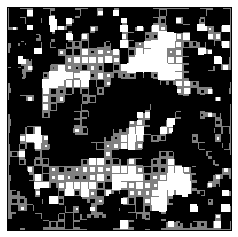
\includegraphics[]{Assets/HINTON1}
    \caption{ Good Hinton Diagram}
    \label{F:TEMP}
    \end{center}
    \end{figure}
    \begin{figure}[]
    \begin{center}
      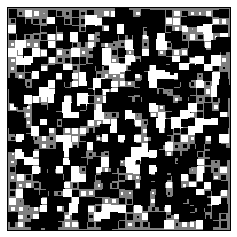
\includegraphics[]{Assets/HINTON2}
    \caption{Bad Hinton Diagram}
    \label{F:TEMP}
    \end{center}
    \end{figure}
